\chapter{Details: SDFDM  model}

%%%%%%%%%%%%%%%%%%%%%%%%%%%%%%%%%%%%%%%%%%%%%% Nij and m_i%%%%%%%%%%%%%%%%%%%%%%%%%%%%%%%%%%%%%%%%%%%%%%%
\section{Analytical formulas for masses and mixing matrix of neutral fermions}
\label{sec:analyt-form-mass}
%
The characteristic equation of the mass matrix~\eqref{eq:Mchi}
is~\cite{Cheung:2013dua}\footnote{The analytical formulas for the neutralino
  masses and the neutralino mixing matrix was
  analyzed in \cite{ElKheishen:1992yv}.}:
\begin{align}
\left[\left({M}^{\chi}_{\text{diag}}\right)_{ii}^2-M_D^2\right]
\left[M_N-\left({M}^{\chi}_{\text{diag}}\right)_{ii}^{\phantom{2}}
\right]
+\tfrac{1}{2}m_{\lambda}^2\left[\left({M}^{\chi}_{\text{diag}}\right)_{ii}+M_D\sin 2\beta
\right]=0\,.
\label{eq:characteristic-equation}
\end{align}
The solutions to the cubic equation in  $\left({M}^{\chi}_{\text{diag}}\right)_{ii}$ are:
\begin{align}
m_1^\chi=&z_2+\dfrac{M_N}{3}\,,&
m_2^\chi=&z_1+\dfrac{M_N}{3}\,, &
m_3^\chi=&z_3+\dfrac{M_N}{3}\,.
\end{align}
where
\begin{align}
z_1&=\left(-\dfrac{q}{2}+\sqrt{\frac{q^2}{4}+\frac{p^3}{27}}\right)^{1/3} + \left(-\dfrac{q}{2}-\sqrt{\dfrac{q^2}{4}+\dfrac{p^3}{27}}\right)^{1/3}\nonumber\\ 
z_2&=-\frac{z_1}{2}+\sqrt{\frac{z_1^2}{4}+\frac{q}{z_1}} \nonumber\\ 
z_3&=-\frac{z_1}{2}-\sqrt{\frac{z_1^2}{4}+\frac{q}{z_1}}\nonumber\\ 
p&=-\frac{1}{3}M_N^2-\left(M_D^2+m_{\lambda}^2\right)  \nonumber\\ 
q&=-\frac{2}{27}M_N^3-\frac{1}{3}M_N\left(M_D^2+m_{\lambda}^2\right)+\left[M_NM_D^2-m_{\lambda}^2\sin(2\beta) M_D\right].
\end{align}

Notice that ${q^2}/{4}+{p^3}/{27} < 0$ and therefore, we have three real masses $m_i^\chi$ $(i=1,2,3)$.

Expanding the eigensystem in Eq.~\eqref{eq:chidiag} by  assuming  that ${N}_{1i}\neq 0$, we have 

\begin{align*}
{M}^{\chi}_{21}\frac{{N}_{2i}}{{N}_{1i}}+{M}^{\chi}_{31}\frac{{N}_{3i}}{{N}_{1i}}&=-({M}^{\chi}_{11}-m_i^\chi)\nonumber \\
({M}^{\chi}_{22}-m_i^\chi)\frac{{N}_{2i}}{{N}_{1i}}+{M}^{\chi}_{32}\frac{{N}_{3i}}{{N}_{1i}}&=-{M}^{\chi}_{12} \nonumber\\
{M}^{\chi}_{23}\frac{{N}_{2i}}{{N}_{1i}}+({M}^{\chi}_{33}-m_i^\chi)\frac{{N}_{3i}}{{N}_{1i}}&=-{M}^{\chi}_{13}\,,
\end{align*}
where
\begin{align}
\label{eq:N1i}
{N}_{1i}=\left[1+\left(\frac{{N}_{2i}}{{N}_{1i}}\right)^2+\left(\frac{{N}_{3i}}{{N}_{1i}}\right)^2\right]^{-1/2}.
\end{align}

Using the matrix $\textbf{M}^{\chi}$ given in the Eq. \eqref{eq:Mchi}, we get the ratios

\begin{align}
\label{eq:exNmn}
\frac{{N}_{2i}}{{N}_{1i}}
&=-\frac{m_{\lambda} \cos\beta}{m_i^\chi}+\frac{M_D}{m_i^\chi}\frac{[m_i^\chi(M_N-m_i^\chi)+m_{\lambda}^2\cos\beta^2 ]}{m_{\lambda}(m_i^\chi\sin\beta +M_D\cos\beta )}\,, \nonumber\\  
\frac{{N}_{3i}}{{N}_{1i}}
&=-\frac{[m_i^\chi(M_N-m_i^\chi)+m_{\lambda}^2 \cos\beta^2]}{m_{\lambda} (m_i^\chi\sin\beta+M_D\cos\beta)}.
\end{align}


\subsection{Approximate mixing matrix}
By using the analytical expressions for the mixing ratios of
Eq.~\eqref{eq:exNmn} with the approximate eigenvalues~\eqref{eq:ml2}
in Eq.~\eqref{eq:N1i}, we obtain

\begin{align}
N_{11}^2=& 1-\frac{\left[M_D^2+M_N^2+2M_DM_N\sin(2\beta)\right]m^2_{\lambda}}{(M_D^2-M_N^2)^2}+\mathcal{O}\left( m_{\lambda}^4 \right)\nonumber\\
N_{12}^2 =&   \frac{[\sin (2 \beta )+1] m_{\lambda }^2}{2 \left(M_N-M_D\right)^2}+\mathcal{O}\left( m_{\lambda}^4 \right)\nonumber\\
N_{13}^2=&  -\frac{[\sin (2 \beta )-1] m_{\lambda }^2}{2 \left(M_D+M_N\right)^2}+\mathcal{O}\left( m_{\lambda}^4 \right)\,.
\end{align}
\begin{align}
N_{21}^2=&\frac{m_{\lambda }^2 \left(\sin\beta  M_D+\cos\beta
   M_N\right)^2}{\left(M_N^2-M_D^2\right)^2}+\mathcal{O}\left( m_{\lambda}^4 \right)\nonumber\\
N_{22}^2=&\frac{1}{2}-\frac{m_{\lambda }^2 (\sin\beta+\cos\beta) \left[\cos\beta M_N-\sin\beta  \left(M_N-2 M_D\right)\right]}{4 M_D \left(M_N-M_D\right)^2}+\mathcal{O}\left( m_{\lambda}^4 \right)\nonumber\\
   N_{23}^2=&\frac{1}{2}+\frac{m_{\lambda }^2 (\cos\beta-\sin\beta) \left[\sin\beta \left(2
   M_D+M_N\right)+\cos\beta M_N\right]}{4 M_D \left(M_D+M_N\right)^2}+\mathcal{O}\left( m_{\lambda}^4 \right).
\end{align}

\begin{align}
\label{eq:mixl2}
N_{31}^2=&\left(\frac{M_{D} \cos\beta + M_{N} \sin\beta}{M_{N}^{2}- M_{D}^{2}} \right)^{2}   m_{\lambda}^{2}
+\mathcal{O}\left( m_{\lambda}^4 \right)\nonumber\\
N_{32}^2=&\frac{1}{2}-\frac{\left[M_{N} \sin\beta - \left( M_{N}- 2 M_{D}\right) \cos\beta\right] \left(\cos\beta+\sin\beta \right)}{4 M_{D} \left(M_{N}- M_{D}\right)^{2}}\,m_{\lambda}^{2}+\mathcal{O}\left( m_{\lambda}^4 \right)  \nonumber\\
N_{33}^2=&\frac{1}{2}- \frac{\left[M_{N} \sin\beta + \left(M_{N} + 2 M_{D}\right) \cos\beta\right] \left(\cos\beta- \sin\beta \right)}{4 M_{D} \left(M_{N} + M_{D} \right)^{2}} \,m_{\lambda}^{2}+\mathcal{O}\left( m_{\lambda}^4 \right).
\end{align}
In particular, with Eq.~\eqref{eq:ml2} and the expressions for $N_{3i}^2$, the identity \eqref{eq:divcan}
is satisfied up to terms of order $\mathcal{O}\left( m_{\lambda}^4
\right)$.










%%%%%%%%%%%%%%%%%%%%%%%%%%%%%%%%%%%%%%%%%%%%%%%%%%%%%%%%%%%%%%%%%%%%%%%%%%%%%%%%%%%%%%%%%%%%%%%%%%%%%%%
\section{The interaction Lagrangian}
\label{sec:lag-interaction}
%
In the SDFDM model we have the next interaction terms (see the Eq.~\ref{eq:lint1})
\begin{align}
\label{eq:lint-weil}
\mathcal{L} = \, & \dfrac{i}{2}\left(
  R_d^{\dagger}\overline{\sigma}^{\mu}D_{\mu}R_d 
+  \widetilde{R}_u^{\dagger}\overline{\sigma}^{\mu}D_{\mu}\widetilde{R}_u \right)
- \dfrac{h}{\sqrt{2}}\left(-\lambda_d\psi_L^0N + \lambda_u{\psi_R^0}^{\dagger}N+\text{h.c}\right)\,,
\end{align}
%
where the field $N$ and the doublets $R_d$, $\widetilde{R}_u$ defined in the Eq.~\ref{eq:weyl-doublets} are constructed of Weyl spinors. 
%
In terms of four-components Dirac spinors constructed with the two-components Weyl spinors $\psi_{LR}^{0,\pm}$ and $N$ as 
%
\begin{align}
\Psi^0=\begin{pmatrix}
\psi_L^0 \\ {\psi_R^0}^{\dagger} 
\end{pmatrix}
\hspace{0.7 cm}
\Psi^{\pm}=\begin{pmatrix}
\psi_L^{\pm} \\ {\psi_R^{\mp}}^{\dagger} 
\end{pmatrix}
\hspace{0.7 cm}
\widetilde{N}=\begin{pmatrix}
N \\ N^{\dagger} 
\end{pmatrix}\,,
\end{align}
%
this Lagrangian can be cast as 
%
\begin{align}
\label{eq:lint-dirac}
\mathcal{L}
=\, & \overline{\Psi}_1i\slashed{D}\Psi_1 + \overline{\Psi}_2 i\slashed{D}\Psi_2
- \dfrac{h}{\sqrt{2}}\left(-\lambda_d\overline{\widetilde{N}}P_L\Psi^0 + \lambda_u \overline{\widetilde{N}}P_R\Psi^0+\text{h.c}\right)\,,
\end{align}
%
where
%
\begin{align}
\Psi_1=\begin{pmatrix}
\Psi_L^0 \\ \Psi_L^-
\end{pmatrix}
\hspace{0.3 cm} , \hspace{0.3 cm}
\Psi_2=\begin{pmatrix}
-\Psi_R^+ \\ \Psi_R^0 
\end{pmatrix}\,
\end{align}
%
are the SU(2)-doublets of Dirac fermions,
%
with $\Psi_{L}^0=P_{L}\Psi^0=(\psi_L^0,0)^{T}$,  $\Psi_{L}^{-}=P_{L}\Psi^{-}=(\psi_L^{-},0)^{T}$, 
$\Psi_{R}^0=P_{R}\Psi^0=(0,{\psi_R^0}^{\dagger})^{T}$ and 
$\Psi_{R}^+=P_{R}\Psi^+ =(0,{\psi_R^-}^{\dagger})^{T}$.
%
Therefore, taking the covariant derivative~\cite{Pich:2005mk}
%
\begin{align}
\label{eq:devcov}
\slashed{D}=&\gamma^{\mu}\left(\partial_{\mu}+ig\widetilde{W}_{\mu}(x)+ig'yB_{\mu}(x)\right)
=\gamma^{\mu}\left(\partial_{\mu}
+ig\dfrac{1}{2}\begin{pmatrix}
W_{\mu}^3 & \sqrt{2}W_{\mu}^{\dagger} \\
\sqrt{2}W_{\mu} & -W_{\mu}^3
\end{pmatrix}
-ig'\dfrac{1}{2} B_{\mu}(x)\right)
\end{align}
%
in the Eq.~\eqref{eq:lint-dirac}, we get explicitly that
%
\begin{align}
\label{eq:kin1}
\overline{\Psi}_1 i\slashed{D}\Psi_1 
=&\bar{R_d}i\gamma^{\mu}\left(\partial_{\mu}
+ig\dfrac{1}{2}\begin{pmatrix}
W_{\mu}^3 & \sqrt{2}W_{\mu}^{\dagger} \\
\sqrt{2}W_{\mu} & -W_{\mu}^3
\end{pmatrix}
-ig'\dfrac{1}{2} B_{\mu}(x)\right)R_d\nonumber\\
=&\begin{pmatrix}
\bar{\Psi}_L^0 & \bar{\Psi}_L^-
\end{pmatrix} i\gamma^{\mu}\left(\partial_{\mu}
+ig\dfrac{1}{2}\begin{pmatrix}
W_{\mu}^3 & \sqrt{2}W_{\mu}^{\dagger} \\
\sqrt{2}W_{\mu} & -W_{\mu}^3
\end{pmatrix}
-ig'\dfrac{1}{2} B_{\mu}(x)\right)\begin{pmatrix}
\Psi_L^0 \\ \Psi_L^-
\end{pmatrix}\nonumber\\
=&\left(\bar{\Psi}_L^0i\slashed{\partial}\Psi_L^0+\bar{\Psi}_L^-i\slashed{\partial}\Psi_L^-\right)
-\dfrac{g}{2}\left[\bar{\Psi}_L^0\gamma^{\mu}W_{\mu}^3\Psi_L^0+\sqrt{2}\bar{\Psi}_L^-\gamma^{\mu}W_{\mu}\Psi_L^0
+\sqrt{2}\bar{\Psi}_L^0\gamma^{\mu}W_{\mu}^{\dagger}\Psi_L^--\bar{\Psi}_L^-\gamma^{\mu}W_{\mu}^3\Psi_L^-\right]
\nonumber\\
+&\dfrac{g'}{2}\left(\bar{\Psi}_L^0\gamma^{\mu}B_{\mu}\Psi_L^0+\bar{\Psi}_L^-\gamma^{\mu}B_{\mu}\Psi_L^-\right)
\nonumber\\
=&\left(\bar{\Psi}_L^0i\slashed{\partial}\Psi_L^0+\bar{\Psi}_L^-i\slashed{\partial}\Psi_L^-\right)
-\dfrac{g}{\sqrt{2}}\left[\bar{\Psi}_L^-\gamma^{\mu}W_{\mu}\Psi_L^0
+\text{h.c}\right] - \dfrac{g}{2}\left[\bar{\Psi}_L^0\gamma^{\mu}W_{\mu}^3\Psi_L^0-\bar{\Psi}_L^-\gamma^{\mu}W_{\mu}^3\Psi_L^-\right]
\nonumber\\
+&\dfrac{g'}{2}\left(\bar{\Psi}_L^0\gamma^{\mu}B_{\mu}\Psi_L^0+\bar{\Psi}_L^-\gamma^{\mu}B_{\mu}\Psi_L^-\right)\nonumber\\
=&\left(\bar{\Psi}_L^0i\slashed{\partial}\Psi_L^0+\bar{\Psi}_L^-i\slashed{\partial}\Psi_L^-\right)
-\dfrac{g}{\sqrt{2}}\left(\bar{\Psi}_L^-\gamma^{\mu}W_{\mu}\Psi_L^0
+\text{h.c}\right)\nonumber\\
-& \dfrac{1}{2}\left[\bar{\Psi}_L^0\gamma^{\mu}(gW_{\mu}^3-g'B_{\mu})\Psi_L^0-\bar{\Psi}_L^-\gamma^{\mu}(gW_{\mu}^3+g'B_{\mu})\Psi_L^-\right]
\nonumber\\
=&\left(\bar{\Psi}_L^0i\slashed{\partial}\Psi_L^0+\bar{\Psi}_L^-i\slashed{\partial}\Psi_L^-\right)
-\dfrac{g}{\sqrt{2}}\left(\bar{\Psi}_L^-\gamma^{\mu}W_{\mu}\Psi_L^0
+\text{h.c}\right)\nonumber\\
-&\dfrac{1}{2}\left[\bar{\Psi}_L^0\gamma^{\mu}\left(\dfrac{g}{\cos\theta_W}Z_{\mu}\right)\Psi_L^0-\bar{\Psi}_L^-\gamma^{\mu}\left(g\left(\dfrac{2\cos^2\theta_W-1}{\cos\theta_W}\right)Z_{\mu}+2eA_{\mu}\right)\Psi_L^-\right]
\nonumber\\
=&\left(\bar{\Psi}_L^0i\slashed{\partial}\Psi_L^0+\bar{\Psi}_L^-i\slashed{\partial}\Psi_L^-\right)
-\dfrac{g}{\sqrt{2}}\left(\bar{\Psi}_L^-\gamma^{\mu}W_{\mu}\Psi_L^0
+\text{h.c}\right)
-\dfrac{g}{2\cos\theta}\bar{\Psi}_L^0\slashed{Z}\Psi_L^0 \nonumber\\
+& g\left(\dfrac{2\cos^2\theta_W-1}{2\cos\theta_W}\right)\bar{\Psi}_L^-\slashed{Z}\Psi_L^--\bar{\Psi}_L^-e\slashed{A}\Psi_L^-\,.
\end{align}
We used the SM relations~\cite{Pich:2005mk}
\begin{align}
g\sin\theta_W=g'\cos\theta_W=e \hspace{0.5 cm} , \hspace{0.5 cm} 
\begin{pmatrix}
Z_{\mu} \\ A_{\mu}
\end{pmatrix}=\begin{pmatrix}
\cos\theta_W & -\sin\theta_W \\
\sin\theta_W & \cos\theta_W
\end{pmatrix}\begin{pmatrix}
W^3_{\mu} \\ B_{\mu}
\end{pmatrix}\,.
\end{align}
%
Analogously
%
\begin{align}
\label{eq:kin2}
\overline{\Psi}_2i\slashed{D}\Psi_2
=&\left(\bar{{\Psi}}_R^0i\slashed{\partial}\Psi_R^0+\bar{\Psi}_R^+i\slashed{\partial}\Psi_R^+\right)
+\dfrac{g}{\sqrt{2}}\left(\bar{\Psi}_R^0\gamma^{\mu}W_{\mu}\Psi_R^+
+\text{h.c}\right)
+\dfrac{g}{2\cos\theta}\bar{\Psi}_R^0\slashed{Z}\Psi_R^0 \nonumber\\
-& g\left(\dfrac{2\cos^2\theta_W-1}{2\cos\theta_W}\right)\bar{\Psi}_R^+\slashed{Z}\Psi_R^+-\bar{\Psi}_R^+e\slashed{A}\Psi_R^+\,.
\end{align}
%
Now, replacing the Eq.~\eqref{eq:kin1} and Eq.~\eqref{eq:kin2} in the Eq.~\eqref{eq:lint-dirac} we have
%
\begin{align}
\label{eq:lint2}
\mathcal{L} =& 
\left(\bar{\Psi}_L^0i\slashed{\partial}\Psi_L^0+\bar{\Psi}_L^-i\slashed{\partial}\Psi_L^-+\bar{{\Psi}_R^0}i\slashed{\partial}
\Psi_R^0+\bar{\Psi}_R^+i\slashed{\partial}\Psi_R^+\right)\nonumber\\
-&\dfrac{g}{\sqrt{2}}\left(\bar{\Psi}_L^-\slashed{W}\Psi_L^0-\bar{\Psi}_R^0\slashed{W}\Psi_R^++\text{h.c}\right)
- \dfrac{g}{2\cos\theta}\left(\bar{\Psi}_L^0\slashed{Z}\Psi_L^0-\bar{\Psi}_R^0\slashed{Z}\Psi_R^0\right) \nonumber\\
+& g\left(\dfrac{2\cos^2\theta_W-1}{2\cos\theta_W}\right)\left(\bar{\Psi}_L^-\slashed{Z}\Psi_L^--\bar{\Psi}_R^+\slashed{Z}\Psi_R^+\right)
-\left(\bar{\Psi}_L^-e\slashed{A}\Psi_L^-+\bar{\Psi}_R^+e\slashed{A}\Psi_R^+\right)
\nonumber\\
-& \dfrac{h}{\sqrt{2}}\left(-\lambda_d\overline{\widetilde{N}}\Psi_L^0 + \lambda_u\overline{\widetilde{N}}\Psi_R^0+\text{h.c}\right)\,.
\end{align}
Therefore, the interaction Lagrangian in the SDFDM model is given by
\begin{align}
\label{eq:lint3}
\mathcal{L}_{\text{Int}} 
=-&\dfrac{g}{\sqrt{2}}\left(\bar{\Psi}_L^-\slashed{W}\Psi_L^0-\bar{\Psi}_R^0\slashed{W}\Psi_R^++\text{h.c}\right)
- \dfrac{g}{2\cos\theta}\left(\bar{\Psi}_L^0\slashed{Z}\Psi_L^0+\bar{\Psi}_R^0\slashed{Z}\Psi_R^0\right) \nonumber\\
+& g\left(\dfrac{2\cos^2\theta_W-1}{2\cos\theta_W}\right)\left(\bar{\Psi}_L^-\slashed{Z}\Psi_L^-+\bar{\Psi}_R^+\slashed{Z}\Psi_R^+\right)
-\left(\bar{\Psi}_L^-e\slashed{A}\Psi_L^-+\bar{\Psi}_R^+e\slashed{A}\Psi_R^+\right)
\nonumber\\
-& \dfrac{h}{\sqrt{2}}\left(-\lambda_d\overline{\widetilde{N}}\Psi_L^0 + \lambda_u\overline{\widetilde{N}}\Psi_R^0+\text{h.c}\right)\,.
\end{align}
%
Finally, we constructed the Majorana spinors $X_i^0$ and  the Dirac spinor $X^{\pm}$  as
\begin{align}
X_i^0=\begin{pmatrix}
(\chi_{i}^0)_\alpha \\ (\chi_i^{0\dagger})^{\dot{\alpha}}
\end{pmatrix}
=\begin{pmatrix}
N_{ji}\,\boldsymbol{\Xi}^{0}_j \\
N_{ji}^{\dagger}\,\boldsymbol{{\Xi}^{\dagger}}^{0}_j
\end{pmatrix}
\hspace{1.5 cm}
X^{\pm}=\begin{pmatrix}
\chi^{\pm}_{\alpha} \\ {\chi^{\mp}}^{\dagger\dot{\alpha}}
\end{pmatrix}
=\begin{pmatrix}
\psi_L^{\pm} \\
{\psi_R^{\mp}}^{\dagger}
\end{pmatrix}\,,
\end{align}
where we used the Eq.~\eqref{eq:vecgauge}. Thus, we can know explicitly the Dirac spinors $\Psi_{LR}^0$ and $\Psi_{LR}^{\pm}$ that we constructed in order to get the Eq.~\eqref{eq:lint3}. Those are
\begin{align}
\Psi_L^0=\begin{pmatrix}
\psi_L^0 \\0
\end{pmatrix}
=N_{2i}\begin{pmatrix}
\chi_i^0 \\ 0
\end{pmatrix}
=N_{2i}P_LX_i^0
\hspace{1.0 cm}
\Psi_R^0=\begin{pmatrix}
0 \\ {{\psi}_R^0}^{\dagger}
\end{pmatrix}=N_{3i}\begin{pmatrix}
0 \\ {\chi_i^0}^{\dagger}
\end{pmatrix}=N_{3i}P_RX_i^0\nonumber
\end{align}
%
\begin{align}
\Psi_L^{\pm}=\begin{pmatrix}
\psi_L^{\pm} \\ 0
\end{pmatrix}=P_LX^{\pm}
\hspace{1.0 cm}
\Psi_R^{\pm}=\begin{pmatrix}
0\\ {\psi_R^{\pm}}^{\dagger}
\end{pmatrix}=P_RX^{\pm}\,.
\end{align}
%
Therefore, replacing these spinors in the Eq.~\eqref{eq:lint3}, we get
\begin{align}
\label{eq:lint4}
\mathcal{L}_{\text{Int}}= & 
-\dfrac{g}{\sqrt{2}}(\bar{X}^-\slashed{W}\left(N_{2i}P_L-N_{3i}P_R\right)X_i^0 + \text{h.c})
+ \dfrac{g}{4\cos\theta}\bar{X}_i^0\slashed{Z}\left(N_{2i}N_{2j}-N_{3i}N_{3j}\right)\gamma^5X_j^0 \nonumber\\
+& g\left(\dfrac{2\cos^2\theta_W-1}{2\cos\theta_W}\right)
\bar{X}^-\slashed{Z}X^-
-e\bar{X}^-\slashed{A}X^- 
-\dfrac{1}{\sqrt{2}}h\bar{X}_i^0\left(-\lambda_dN_{2i}N_{1j} + \lambda_uN_{3i}N_{1j}\right)X_j^0\,,
\end{align}
i.e. the interaction of the DM with de $W$, $Z$ and $h$ SM gauge boson is given by
\begin{align}
\mathcal{L^{\chi}}_{\text{Int}}=-\bar{X}^-\slashed{W}c_{WXX_i}X_i^0
-c_{ZX_iX_j}Z_{\mu}\bar{X}_i^0\gamma^{\mu}\gamma^{5}X_j^0
-c_{hX_iX_j}h\bar{X}_i^0X_j^0
\end{align}
where 
\begin{align}
c_{WXX_i}=& \dfrac{g}{\sqrt{2}}\left(N_{2i}P_L-N_{3i}P_R\right)  \label{eq:cWXXi}\\
c_{ZX_iX_j}=&\frac{g}{4\cos\theta_W}(N_{3i}N_{3j}-N_{2i}N_{2j}) \label{eq:cZXiXj}\\
%problema en el orden
c_{hX_iX_j}=&\frac{1}{\sqrt{2}}(-\lambda_dN_{2i}N_{1j}+\lambda_uN_{3i}N_{1j})\label{eq:cHXiXj}\,.
\end{align}










%%%%%%%%%%%%%%%%%%%%%%%%%%%%%%%%%%%%%% AMPLITUDE SI CROSS SECTION %%%%%%%%%%%%%%%%%%%%%%%%%%%%%%%%%%%%%%%%%
\section{Spin-independent cross section in the SDFDM model}
\label{sec:SI-amplitude}
%
\begin{figure}[h]
  \centering
  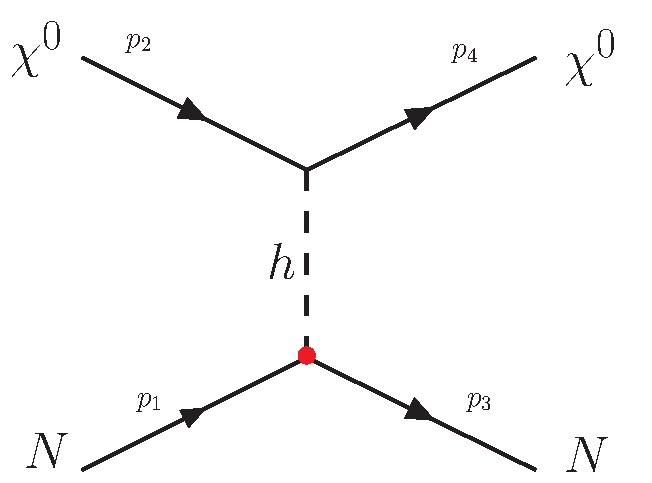
\includegraphics[scale=0.45]{SI_N}
  \caption{Scalar elastic scattering with nucleons.}
  \label{fig:SI_N}
\end{figure}
%
The amplitude of the process shown in Fig.~\ref{fig:SI_N} is
\begin{align}
\mathcal{M}=&\bar{u}(s_3,p_3)u(s_1,p_1)\dfrac{im_Nf_N}{v}i\Delta_F(p_1-p_3)ic_{hX_1X_1}\bar{u}(s_4,p_4)u(s_2,p_2)\nonumber\\
=& -i\dfrac{im_Nf_N}{v}c_{hX_1X_1}\Delta_F(p_1-p_3) \bar{u}(s_3,p_3)u(s_1,p_1)\bar{u}(s_4,p_4)u(s_2,p_2)\,,
\end{align}
therefore,
\begin{align}
\sum_{s_i}|\mathcal{M}|^2=&\left(\dfrac{m_Nf_N}{v}c_{hX_1X_1}\Delta_F(p_1-p_3)\right)^2
\sum_{s_{1,3}}\left(\bar{u}_{s_3p_3}u_{s_1p_1}\right)\left(\bar{u}_{s_3p_3}u_{s_1p_1}\right)^{\dagger}
\sum_{s_{2,4}}\left(\bar{u}_{s_4p_4}u_{s_2p_2}\right)\left(\bar{u}_{s_4p_4}u_{s_2p_2}\right)^{\dagger}\nonumber\\
=&\left(\dfrac{m_Nf_N}{v}c_{hX_1X_1}\Delta_F(p_1-p_3)\right)^2
\sum_{s_{1,3}}\left(\bar{u}_{s_3p_3}u_{s_1p_1}\bar{u}_{s_1p_1}u_{s_3p_3}\right)
\sum_{s_{2,4}}\left(\bar{u}_{s_4p_4}u_{s_2p_2}\bar{u}_{s_2p_2}u_{s_4p_4}\right)\nonumber\\
=&\left(\dfrac{m_Nf_N}{v}c_{hX_1X_1}\Delta_F(p_1-p_3)\right)^2
\text{Tr}\left[(\slashed{p}_1+m_N)(\slashed{p}_3+m_N)\right]
\text{Tr}\left[(\slashed{p}_2+m_{\chi^0})(\slashed{p}_4+m_{\chi^0})\right]\nonumber\\
=&\left(\dfrac{m_Nf_N}{v}c_{hX_1X_1}\Delta_F(p_1-p_3)\right)^2
\left(4p_1\cdot p_3+4m_N^2\right)\left(4p_2\cdot
p_4+4m_{\chi^0}^2\right)\,.
\end{align}
Now, if we do the approximation of $p_i\to0$, we get
\begin{align}
\overline{|\mathcal{M}|^2}=\sum_{s_i}|\mathcal{M}|^2\approx&\left(\dfrac{m_Nf_N}{v}c_{hX_1X_1}\dfrac{1}{m_h^2}\right)^2 16m_N^2m_{\chi^0}^2
=\dfrac{16f_N^2c_{hX_1X_1}^2m_N^4m_{\chi^0}^2}{v^2m_h^4}\,.
\end{align}
Therefore, it means that for an elastic scattering, the differential cross section is given by
\begin{align}
\dfrac{d\sigma}{d\Omega}=\dfrac{1}{64\pi^2 s}\overline{|\mathcal{M}|^2}
\approx\dfrac{1}{64\pi^2 (m_N+m_{\chi^0}^2)^2}\dfrac{16f_N^2c_{hX_1X_1}^2m_N^4m_{\chi^0}^2}{v^2m_h^4}
=\dfrac{m_r^2}{4\pi^2}\left(\dfrac{c_{hX_1X_1}}{vm_h^2}\right)^2f_N^2m_N^2\,,
\end{align}
where $s=(E_N+E_{\chi^0})^2\approx(m_N+m_{\chi^0})^2$ in the limit of zero-momentum and $m_r=\dfrac{m_Nm_{\chi^0}}{(m_N+m_{\chi^0})}$ is the reduced mass of the system.
%
Finally, integrating in the solid angle, the spin-independent cross section a tree level is given by
\begin{align}
\label{eq:SI-tree-level}
\sigma_{SI}=\dfrac{m_r^2}{\pi}\left(\dfrac{c_{hX_1X_1}}{vm_h^2}\right)^2f_N^2m_N^2\,.
\end{align}
% 












%%%%%%%%%%%%%%%%%%%%%%%%%%%%%%%%%%%%%%%%%%%%%%%%%%%%%%%%%%%%%%%%%%%%%%%%%%%%%%%%%%%%%%%%%%%%%%%%%%%%%%%%%%%%
\section{One-loop neutrino masses in the interaction basis}
\label{sec:mass-interaction-basis}

By using the Feynman rules for Weyl spinors we have the diagrams for
neutrino masses at one-loop shown in \ref{fig:t13aweyl}
%
\begin{figure}[h]
  \centering
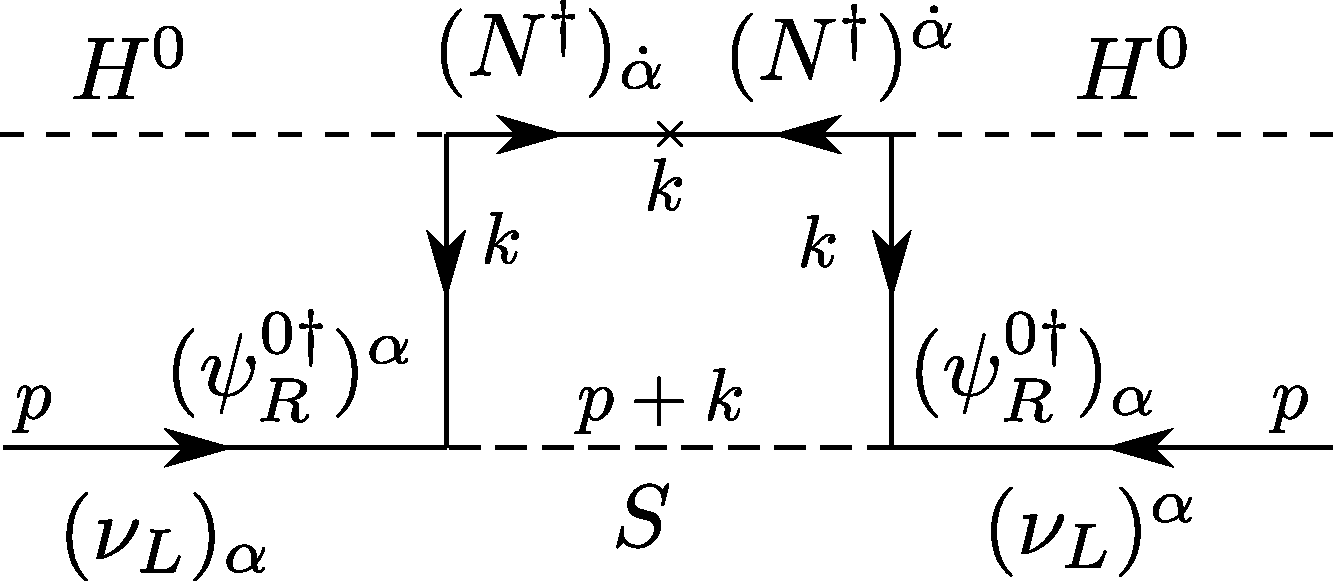
\includegraphics[scale=0.3]{T13AweylR}\qquad 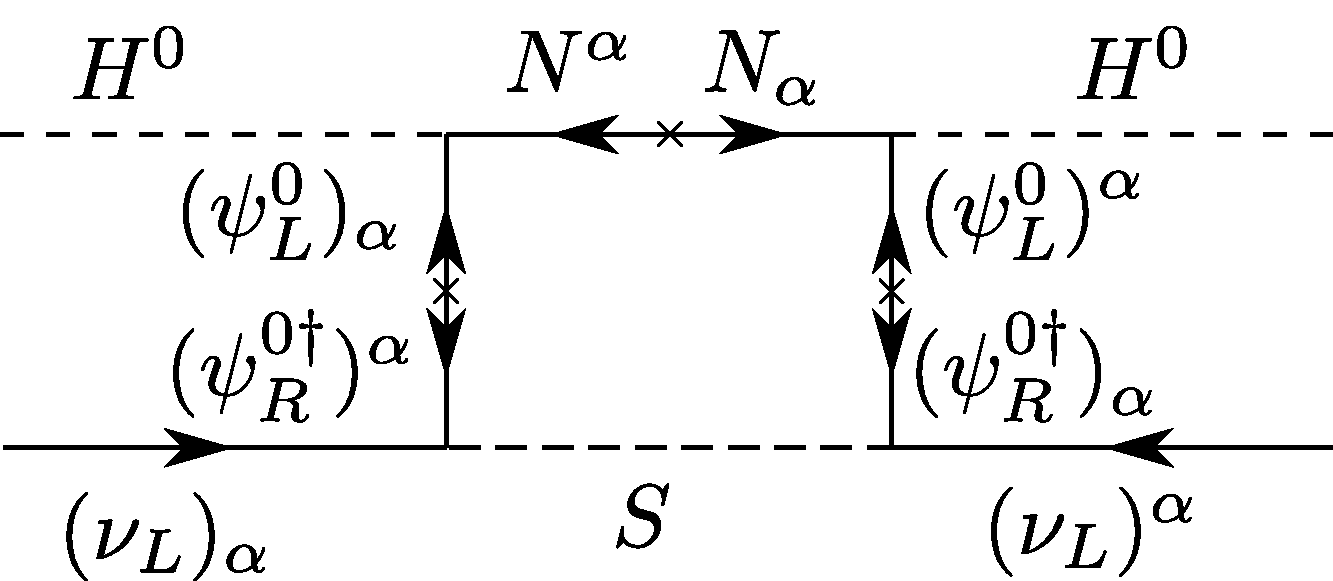
\includegraphics[scale=0.3]{T13AweylRL}
  \caption{One-loop neutrino mass in the interaction basis}
  \label{fig:t13aweyl}
\end{figure}

The results from the Refs.~\cite{Bonnet:2012kz,Suematsu:2010nd} adapted to our case imply that ($\lambda_d \to Y_L\; \lambda_u \to Y_R$)
%check nuint.pdf
\begin{align}
  M^{\nu}_{ij}=2\sum_{\alpha}h_{i\alpha}h_{j\alpha} &\left[  \lambda_u^2\int \frac{d^4 k}{(2\pi)^4}i S_F \left(k,M_D \right)P_R S_F \left(k,M_N \right)P_R i S_F \left(k,M_D \right)
             \Delta_F \left( k+p,m_{S_\alpha} \right)\right. \nonumber\\
          &\left.+\lambda_d^2\int \frac{d^4 k}{(2\pi)^4}i S_F \left(k,M_D \right)P_L S_F \left(k,M_N \right)P_L i S_F \left(k,M_D \right)
             \Delta_F \left( k+p,m_{S_\alpha} \right) 
            \right].
\end{align}

\begin{align}
  M^{\nu}_{ij}=\sum_{\alpha}\frac{2h_{i\alpha}h_{j\alpha}v^2 M_N}{(4\pi)^2} 
      \left[\lambda_u^{2} \, J_4\left(M_D^2,M_D^2,M_N^2,m^{S}_{\alpha}  \right)
            + \lambda_d^2 M_D^2  \, I_4\left(M_D^2,M_D^2,M_N^2,m^2_{S_\alpha}  \right)
      \right],
\end{align}
where
\begin{align}
   J_4\left(M_D^2,M_D^2,M_N^2,m^2_{S}  \right)=&\frac{(4\pi)^2}{i}
   \int \frac{d^4 k}{(2\pi)^4}
\frac{k^2}{\left(k^2-m_D^2\right)^2\left( k^2-M_N^2 \right)\left(k^2-m_{S_\alpha}^2\right)} \nonumber\\
   I_4\left(M_D^2,M_D^2,M_N^2,m^2_{S}  \right)=&\frac{(4\pi)^2}{i}
   \int \frac{d^4 k}{(2\pi)^4}
\frac{1}{\left(k^2-m_D^2\right)^2\left( k^2-M_N^2 \right)\left(k^2-m_{S_\alpha}^2\right)}.
\end{align}
After integration
%see calculoij.pdf
\begin{align*}
  J_4\left(M_D^2,M_D^2,M_N^2,m^2_{S}  \right)=
-&\left\{  \left[\frac{M_D^2}{\left(M_N^2-M_D^2\right)\left(m_{S}^2-M_D^2\right)} 
-\frac{M_D^4 \left(2M_D^2-M_N^2-m_{S_\alpha}^2\right)}{2\left(M_N^2-M_D^2\right)^2\left(m_{S}^2-M_D^2\right)^2} \right]\ln M_D^2\right.\nonumber\\
&-\frac{M_N^4\ln M_N^2}{2\left( m_{S_\alpha}^2-M_N^2 \right)\left( M_D^2-M_N^2 \right)^2}-
\frac{m_{S_\alpha}^4\ln m_{S_\alpha}^2}{2\left( m_N^2-m_{S_\alpha}^2 \right)\left( M_D^2-m_{S_\alpha}^2 \right)^2}
\nonumber\\
 &\left.+\frac{M_D^2}{2\left(M_N^2-M_D^2  \right)\left(m_{S_\alpha}^2-M_D^2  \right)} \right\},
\end{align*}
\begin{align}
      I_4&\left(M_D^2,M_D^2,M_N^2,m^2_{S}  \right)=\nonumber\\
&\left[\frac{M_N^2\ln \left( M_N^2/M_D^2 \right)}{\left( M_N^2-M_D^2 \right)^4\left( M_N^2-m_{S_\alpha}^2 \right)^2}
      -\frac{m_{S_\alpha}^2\ln \left( m_{S_\alpha}^2/M_D^2 \right)}{\left( m_{S_\alpha}^2-M_D^2 \right)^4\left( M_N^2-m_{S_\alpha}^2 \right)^2}-
      \frac{1}{\left(m_{S_\alpha}^2-M_D^2\right)^2\left(M_N^2 -M_D^2 \right)^2} 
 \right],
\end{align}
or
\begin{align}
   I_4\left(M_D^2,M_D^2,M_N^2,m^2_{S}  \right)=
-&\left[ \frac{\left(M_D^4-M_N^2 m_{S_\alpha}^2\right)\ln M_D^2}{\left(M_N^2 -M_D^2 \right)^2\left(m_{S_\alpha}^2 -M_D^2 \right)^2} 
+\frac{M_N^2 \ln M_N^2}{\left(m_{S_\alpha}^2 -M_N^2 \right)\left(M_D^2-M_N^2\right)^2}\right. \nonumber\\
&\left.+\frac{m_{S_\alpha}^2 \ln m_{S_\alpha}^2}{\left(M_N^2 -m_{S_\alpha}^2 \right)\left(M_D^2-m_{S_\alpha}^2\right)^2} 
-\frac{1}{\left(m_{S_\alpha}^2-M_D^2\right)\left(M_N^2 -M_D^2 \right)} 
\right].
\end{align}
%
In  the Ref.~\cite{Fraser:2014yha} only the contribution proportional to $\lambda_u$ is considered in the limit $M_N\to 0$~\footnote{$\lim_{x\to 0}x\ln x=\lim_{x\to 0}\dfrac{\ln x}{1/x}=0$}, 
\begin{align*}
   J_4\left(M_D^2,M_D^2,M_N^2,m^2_{S}  \right)=&
-\left\{  \left[-\frac{M_D^2}{M_D^2\left(m_{S}^2-M_D^2\right)} 
-\frac{M_D^4 \left(2M_D^2-m_{S_\alpha}^2\right)}{2M_D^4\left(m_{S}^2-M_D^2\right)^2} \right]\ln M_D^2\right.\nonumber\\
&\qquad+\frac{m_{S_\alpha}^4\ln m_{S_\alpha}^2}{2m_{S_\alpha}^2\left( M_D^2-m_{S_\alpha}^2 \right)^2} 
\left.-\frac{M_D^2}{2M_D^2\left(m_{S_\alpha}^2-M_D^2  \right)} \right\}\nonumber\\
=&  -\left\{  -\left[\frac{1}{\left(m_{S}^2-M_D^2\right)} 
+\frac{\left(2M_D^2-m_{S_\alpha}^2\right)}{2\left(m_{S}^2-M_D^2\right)^2} \right]\ln M_D^2
+\frac{m_{S_\alpha}^2\ln m_{S_\alpha}^2}{2\left( M_D^2-m_{S_\alpha}^2 \right)^2} 
-\frac{1}{2\left(m_{S_\alpha}^2-M_D^2  \right)} \right\}\nonumber\\
=&  -\frac{1}{\left(m_{S}^2-M_D^2\right)}\left\{  -\left[1 
+\frac{\left(2M_D^2-m_{S_\alpha}^2\right)}{2\left(m_{S}^2-M_D^2\right)} \right]\ln M_D^2
+\frac{m_{S_\alpha}^2\ln m_{S_\alpha}^2}{2\left( M_D^2-m_{S_\alpha}^2 \right)} 
-\frac{1}{2} \right\}\nonumber\\
= & \frac{1}{2\left(m_{S}^2-M_D^2\right)}\left\{  \frac{m_{S_\alpha}^2\ln M_D^2}{\left(m_{S}^2-M_D^2\right)}
-\frac{m_{S_\alpha}^2\ln m_{S_\alpha}^2}{\left( M_D^2-m_{S_\alpha}^2 \right)} +1 \right\}\nonumber\\
=&  \frac{1}{2\left(m_{S}^2-M_D^2\right)}\left[ 1+ \frac{m_{S_\alpha}^2\ln \left( M_D^2/m_{S_\alpha}^2 \right)}{\left(m_{S}^2-M_D^2\right)}
\right]\nonumber\\
=& - \frac{1}{2\left(M_D^2-m_{S}^2\right)}\left[ 1-\frac{m_{S_\alpha}^2\ln \left( M_D^2/m_{S_\alpha}^2 \right)}{\left(M_D^2-m_{S}^2\right)}
\right].
\end{align*}
So that
\begin{align*}
M^{\nu}_{ij}=-\sum_{\alpha}\frac{h_{i\alpha}h_{j\alpha}\left(\lambda_u^2 v^2\right)M_N}{16\pi^2\left(M_D^2-m_{S_\alpha}^2\right)}
\left[ 1-\frac{m_{S_\alpha}^2\ln \left( M_D^2/m_{S_\alpha}^2 \right)}{\left(M_D^2-m_{S_\alpha}^2\right)}\right].
\end{align*}









%%%%%%%%%%%%%%%%%%%%%%%%%%%%%%%%%%%%%%%%%%%%%%%%%%%%%%%%%%%%%%%%%%%%%%%%%%%%%%%%%%%%%%%%%%%%%%%%%%%%%%%%%
\section{$\mu  \rightarrow e \gamma$ process in the SDFDM model with real scalars singlets}
\label{sec:Ap-muegamma}

The $\mu  \rightarrow e \gamma$ process in this model is shown in Fig.~\ref{fig:muegamma}.
In general, the radiative decay $f_1(p_1)  \rightarrow f_2(p_2) \gamma (q)$, where, $q=p_1-p_2$, $f_1$ has a mass $m_1$ and $f_2 $ has a mass $m_2$ was computed in the Ref.~\cite{Lavoura:2003xp}. Here, we adapt their analysis to our model.

We take the fermions on shell, i.e. $p_1^2=m_1^2$  and $p_2^2=m_2^2$ and they are represented by spinors $u_1$ and $u_2$, which satisfy the relations $\cancel{p}_1u_1=m_1u_1$ and $\bar{u}_2\cancel{p}_2=m_2\bar{u}_2$.
%
The amplitude for the decay is given by $e \epsilon^*_{\mu}(q)M^{\mu}$, where $\epsilon^*_{\mu}(q)$ is the outgoing photon polarization and $e$ is the electric charge of the electron. We know that the gauge invariance implies that $q_{\mu}M^{\mu}$ must be zero. 
Therefore, $M^{\mu}$ has the form
%\begin{align}
%M^{\mu}=\bar{u}_2(p_2)( \sigma_L\Sigma_L^{\mu}+\sigma_R\Sigma_R^{\mu} +\mathcal{O}^{\mu} )u_1(p_1)\,,
%\end{align}
%where
%\begin{align}
%\Sigma_L^{\mu}=&(p_1^{\mu}+p_2^{\mu})P_L-\gamma^{\mu}(m_2P_L+m_1P_R)\\	
%\Sigma_R^{\mu}=&(p_1^{\mu}+p_2^{\mu})P_R\gamma^{\mu}(m_2P_R+m_1P_L)\,.
%\end{align}
%%
%We only take care of $\sigma_{L}$ and $\sigma_{R}$ factors, not for $\mathcal{O}^{\mu}$, because they are the only relevant parameters important for $f_1 \rightarrow f_2 \gamma$ decay and on-shell photon. Therefore, we will not put the $\mathcal{O}^{\mu}$ term anymore.
%
%Alternatively, we can write $M^{\mu}$ in the form
\begin{align}
M^{\mu}=\bar{u}_2(p_2)( i\sigma^{\mu\nu}q_{\nu}(\sigma_LP_L+\sigma_RP_R))u_1(p_1)\,,
\end{align}
%
and the partial width for the process $f_1\rightarrow f_2\gamma$ is given by
%
\begin{align}
\Gamma = \dfrac{(m_1^2-m_2^2)^3(|\sigma_L|^2+|\sigma_R|^2)}{16\pi m_1^3}\,.
\label{partial_width_muegamma}
\end{align}
%
With all this in mind, our work is determinate the $\sigma_L$ and the $\sigma_R$ factors in this model and use the general Eq.~\eqref{partial_width_muegamma} for the partial width of this process.

In general, for a Yukawa Lagrangian
%
\begin{align}
\label{eq:general-yukawa-lagrangian}
\mathcal{L}_{\text{Yukawa}}=B\overline{F}(L_iP_L+R_iP_R)f_i+B^*\overline{f}_i(L_i^*P_R+R_i^*P_L)F\,,
\end{align}
where the fermions $f_i$ have charge $Q_f=e$, the boson $B$ have charge $Q_B$ and the fermions $f_i$ have interaction with the boson $B$ and fermion $F$ with arbitrary dimensionless numerical coefficients $L_i$ and $R_i$, the $\sigma_L$ and $\sigma_R$ factors are given by
\begin{align}
\label{eq:sigma-L}
\sigma_L=& Q_f(\rho k_1 +\lambda k_2 + v k_3)+Q_B(\rho \overline{k}_1 + \lambda \overline{k}_2 + v \overline{k}_3)\\
\label{eq:sigma-R}
\sigma_R=& Q_f(\lambda k_1 +\rho k_2 + \zeta k_3)+Q_B(\lambda \overline{k}_1 + \rho \overline{k}_2 + \zeta \overline{k}_3)\,,
\end{align} 
where
%
\begin{align}
\lambda=&L_2^+L_1 \hspace{2.0 cm} k_1=m_1(c_1+d_1+f) \hspace{2.0 cm} \overline{k}_1=m_1(-\overline{c}_1+\overline{d}_1+\overline{f}) \nonumber\\
\rho=&R_2^*R_1    \hspace{2.0 cm} k_2=m_2(c_2+d_2+f) \hspace{2.0 cm} \overline{k}_2=m_2(-\overline{c}_2+\overline{d}_2+\overline{f}) \nonumber\\
\zeta=&L_2^*R_1   \hspace{2.0 cm} k_3=m_F(c_1+c_2)   \hspace{2.7 cm} \overline{k}_3=m_F(-\overline{a}+\overline{c}_1+\overline{c}_2)  \nonumber\\
v=&R_2^*L_1 \,.
\end{align}

\subsubsection{$\sigma_L$ and $\sigma_R$ in SDFDM model}

For our specify case, the Yukawa Lagrangian included in the Eq.~\ref{eq:lt13a} is given by
\begin{align}
\mathcal{L}_{\text{Yukawa}}^{\text{SDFDM}}&=\, h_{i\alpha}\overline{e_{Li}}\psi^-_{R}S_\alpha+ \text{h.c} =S_\alpha\overline{\psi^-}[h_{i\alpha}P_L]e_i + S_\alpha\overline{e_i}[h_{i\alpha}P_R]\psi^- \,.
\end{align}
%
Therefore, we can do the next identification with the Lagrangian~\ref{eq:general-yukawa-lagrangian}
%
\begin{center}
\begin{tabular}{|l|l|l|l|}
\hline
B $\rightarrow S_\alpha$ & $R_i \rightarrow  0$ & $R_i^* \rightarrow  h_{i\alpha}$  & $Q_B=0$\\
F $\rightarrow \psi^-$ & $L_i \rightarrow h_{i\alpha}$ & $L_i^* \rightarrow  0$ &$Q_F=1$ \\
$f_i \rightarrow e_{i}$ &  &  & \\ 
\hline
\end{tabular}\,.
%
\end{center}
Replacing these factors in the Eq.~\eqref{eq:sigma-L} and Eq.~\eqref{eq:sigma-R} we get that
\begin{align}
\sigma_L=&eh_{2\alpha}h_{1\alpha}m_1(c_1+d_1+f)=eh_{2\alpha}h_{1\alpha}m_1(c_1+\dfrac{3}{2}d) \nonumber\\
\sigma_R=&eh_{2\alpha}h_{1\alpha}m_2(c_2+d_2+f)=eh_{2\alpha}h_{1\alpha}m_2(c_2+\dfrac{3}{2}d) \approx 0 \,.
\label{sigmas}
\end{align}
%
In the last equation, the relations $d_1=d_2=2f=d$, and $m_1=m_{\mu} \gg m_2=m_{e} $ were used.

According with the Ref.~\cite{Lavoura:2003xp}, the parameters $c_i=c$ and $d_i=d$ are related with the loop integrals as follows
\begin{align}
\bigg(c+\dfrac{3}{2}d\bigg)=&\dfrac{i}{16\pi^2 m_B^2}\bigg[\dfrac{x^2-5x-2}{12(x-1)^3}+\dfrac{x \ln x}{2(x-1)^4}\bigg]=\dfrac{i}{16\pi^2 m_B^2}\dfrac{1}{2}\bigg[\dfrac{x^3-6x^2+3x+2+6x\ln x}{6(x-1)^4}\bigg]\,,
\end{align}
where $x=m_F^2/m_{\phi}^2 $. 

Finally, putting all this in the Eq.~\eqref{sigmas} we get the relations
\begin{align}
\sigma_L=&\dfrac{i eh_{2\alpha}h_{1\alpha}m_{\mu}}{16\pi^2 m_B^2}\dfrac{1}{2}F(x)\nonumber \\
\sigma_R \approx & 0 \,,
\label{sigmas_result}
\end{align}
where
\begin{align}
F(x)=\bigg[\dfrac{x^3-6x^2+3x+2+6x\ln x}{6(x-1)^4}\bigg] \hspace{1 cm} \text{with} \hspace{1 cm} x=\dfrac{M_D^2}{m_{S_{\alpha}}^2}\,.
\label{Fx}
\end{align}

\subsubsection{ Branching ($\mu \rightarrow e \gamma$)}
Putting the Eq.~\eqref{sigmas_result} into the Eq.~\eqref{partial_width_muegamma} we get
\begin{align}
\Gamma =&\dfrac{(m_{\mu}^2-m_e^2)^3}{16\pi m_{\mu}^3}(|\sigma_L|^2) \approx \dfrac{m_{\mu}^3 |\sigma_L|^2}{16\pi}
= \dfrac{m_{\mu}^5}{16\pi}\bigg| \dfrac{e h_{1\alpha}h_{2\alpha}}{16 \pi^2 m_{S_\alpha}^2} \dfrac{F(x)}{2} \bigg|^2\,.
\end{align}
Therefore, the branching ratio for this process is given by
\begin{align}
\operatorname{Br}(\mu \rightarrow e \gamma) 
=& \dfrac{\Gamma(\mu \rightarrow e \gamma )}{\Gamma(\mu \rightarrow e \bar{\nu}_e \nu_{\mu})}
=\dfrac{\dfrac{m_{\mu}^5}{16\pi}\bigg| \dfrac{e h_{1\alpha}h_{2\alpha}}{16 \pi^2 m_{S_\alpha}^2} \dfrac{F(x)}{2} \bigg|^2}{ \dfrac{G_F^2 m_{\mu}^5}{192\pi^3} }
=\dfrac{3}{4}\dfrac{1}{G_F^2}\bigg(\dfrac{e^2}{4\pi}\bigg)\dfrac{1}{16\pi}\bigg|\dfrac{F(x)h_{1\alpha}h_{2\alpha}}{m_{S_\alpha}^2}\bigg|^2 \nonumber \\
=&\dfrac{3}{4}\dfrac{\alpha_{em}}{16 \pi G_F^2}\left|\sum_{\alpha}\dfrac{F(x)h_{1\alpha}h_{2\alpha}}{m_{S_\alpha}^2}  \right|^2 \,.
%\label{branching_muegamma}
\end{align}
%
In general, for a complex Yukawa coupling $h_{i\alpha}$ we have,
\begin{align}
\operatorname{Br}(\mu \rightarrow e \gamma)=&\dfrac{3}{4}\dfrac{\alpha_{\text{em}}}{16 \pi G_F^2}\left|\sum_{\alpha}
h_{1\alpha}\frac{F\left(M_D^2/m_{S_{\alpha}}^2  \right) }{m_{S_\alpha}^2}h_{2\alpha}^{*}  \right|^2 \,.
\end{align}











